% IPP
% Projekt - 1.
% Juraj Holub
% xholub40@stud.fit.vutbr.cz

\documentclass[a4paper, 10pt]{article}
\usepackage[utf8]{inputenc}
\usepackage[english]{babel}
\usepackage[T1]{fontenc}
\usepackage[left=2cm,top=2.5cm, right=2cm]{geometry}
\usepackage{hyperref}
\usepackage{graphicx}
\usepackage{float}

\title{Documentation of Project Implementation for IPP 2018/2019 }
\author{Name and surname: Juraj Holub\\ Login: xholub40}
\date{}

\begin{document}
	\maketitle
	\thispagestyle{empty}

% proposal of solution
\section{Proposal of solution} \label{proposal}


\begin{figure}[H] 
	\centering
	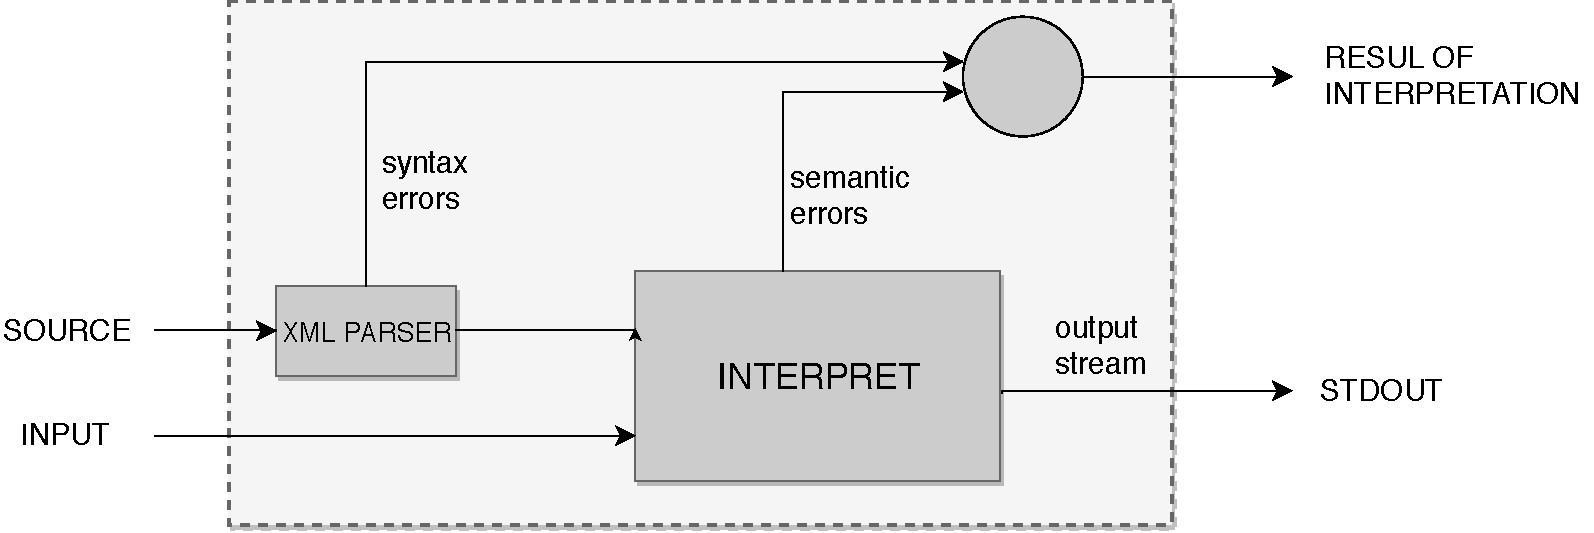
\includegraphics[width=.8 \paperwidth]{interpret.pdf}
	\caption{Scheme of implemented interpretation solution.}
	\label{obr1}
\end{figure} 

Figure \ref{obr1} shows scheme of implemented algorithm of parsing IPPcode19 and generating XML output.

\section{Implementation details}
Suggested solution parted to three blocks described in section \ref{proposal} is implemented in three logical units:
\begin{itemize}
	\item \textbf{XML parser}: parse input file to xml, using ElementTree, syntax check
	\item \textbf{Interpret}: 
	\item \textbf{Error handling}: 
	\item \textbf{String convertor}:  
\end{itemize}



\end{document}
